% Generated by pysimcount.figleader -- do not edit; regenerate instead.
% figure: bound-min-t-all-formulas -- cost at n = 500, one row per formula
% seeds [1, 2, 3, 4, 5, 6, 7, 8, 9, 10]; metric=t kind=xyz merged (Clifford+T (ct), simcount template)
% shown: suzuki2, suzuki4, mo-q6, mo-q14, bm-q10, mo-o8-q21, morales-y8m10, morales-m8
% removed (see bound-min-t-all-formulas-ranking.md): lie-trotter, suzuki6, suzuki8
% n = 500; r from minimised norm bound (Childs et al. 2018, Def. 2; extended to every formula); x = mean over seeds, bars min..max over seeds
% cheapest on = seeds on which the formula is cheapest; rank range = min..max of its rank over seeds
% derived: bound-min-t-all-formulas.json by pysimcount.figleader; source_sha256=a4b15e4708c194b9d2867c8e4268e5b0434b28c9977d4aa360fb0b7e04741962
% figure made at git_commit=eed0c490bd2a7ed3c821acf76ae930c79d2195f6 git_dirty=True
% WARNING: made from uncommitted code; the commit above does not reproduce it.
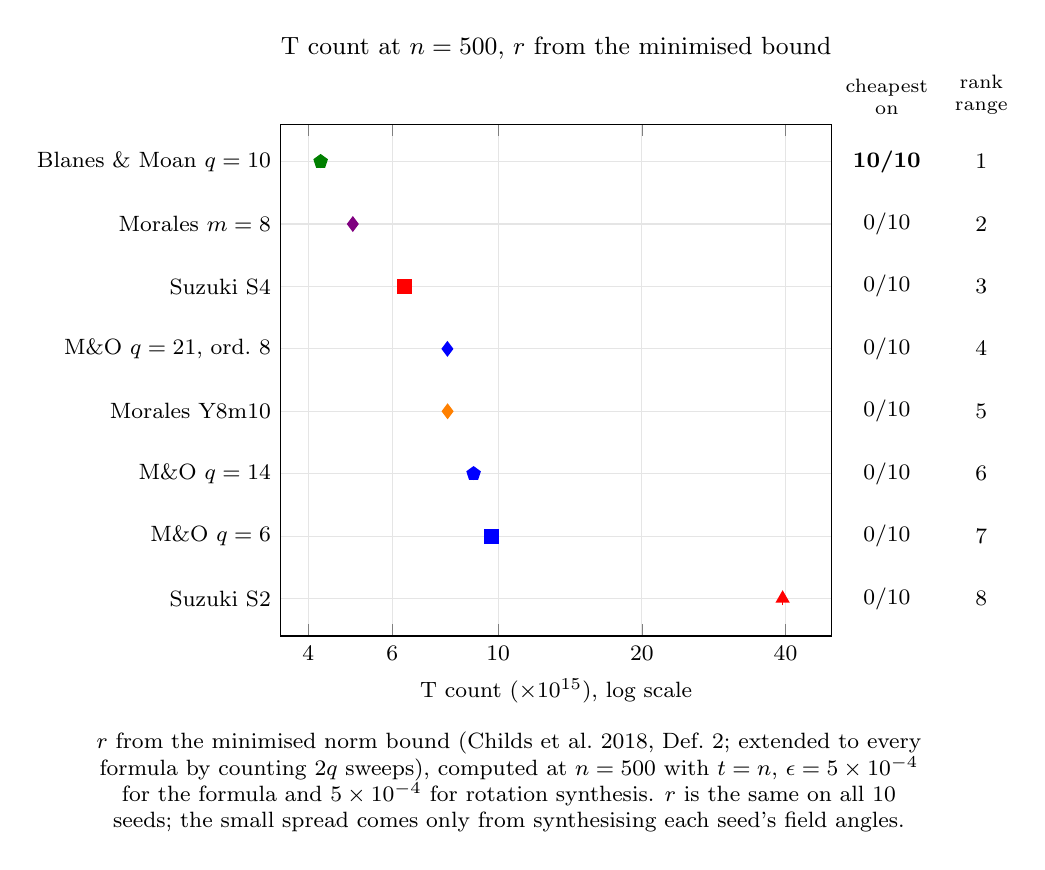
\begin{tikzpicture}
  \begin{semilogxaxis}[
    scale only axis, clip=false,
    at={(0cm,0cm)}, anchor=south west,
    width=7.0cm, height=6.5cm,
    title={T count at $n = 500$, $r$ from the minimised bound}, title style={font=\small, yshift=14pt},
    xlabel={T count ($\times 10^{15}$), log scale}, xlabel style={font=\footnotesize},
    xmin=3.5e+15, xmax=5e+16, xtick={4e+15,6e+15,1e+16,2e+16,4e+16}, xticklabels={4,6,10,20,40},
    xminorticks=false,
    y dir=reverse, ymin=0.4, ymax=8.6, ytick={1,2,3,4,5,6,7,8},
    yticklabels={{Blanes \& Moan $q=10$},{Morales $m=8$},{Suzuki S4},{M\&O $q=21$, ord.~8},{Morales Y8m10},{M\&O $q=14$},{M\&O $q=6$},{Suzuki S2}},
    tick label style={font=\footnotesize}, ytick style={draw=none},
    xmajorgrids=true, ymajorgrids=true, grid style={black!10},
  ]
    % bm-q10: plotted 4.24434e+15, seeds 4.24386e+15..4.24465e+15, cheapest on 10/10, rank 1..1
    \addplot[green!50!black, only marks, mark=pentagon*, mark size=2.4pt, mark options={solid, fill=green!50!black, line width=0.6pt}, error bars/.cd, x dir=both, x explicit, error bar style={solid, line width=0.6pt}] coordinates {
      (4.24434e+15,1) += (3.04117e+11,0) -= (4.77675e+11,0)
    };
    % morales-m8: plotted 4.9572e+15, seeds 4.9569e+15..4.95749e+15, cheapest on 0/10, rank 2..2
    \addplot[violet, only marks, mark=diamond*, mark size=2.4pt, mark options={solid, fill=violet, line width=0.6pt}, error bars/.cd, x dir=both, x explicit, error bar style={solid, line width=0.6pt}] coordinates {
      (4.9572e+15,2) += (2.92503e+11,0) -= (2.97895e+11,0)
    };
    % suzuki4: plotted 6.36193e+15, seeds 6.36115e+15..6.36276e+15, cheapest on 0/10, rank 3..3
    \addplot[red, only marks, mark=square*, mark size=2.4pt, mark options={solid, fill=red, line width=0.6pt}, error bars/.cd, x dir=both, x explicit, error bar style={solid, line width=0.6pt}] coordinates {
      (6.36193e+15,3) += (8.36818e+11,0) -= (7.81907e+11,0)
    };
    % mo-o8-q21: plotted 7.82549e+15, seeds 7.82487e+15..7.82623e+15, cheapest on 0/10, rank 4..4
    \addplot[blue, only marks, mark=diamond*, mark size=2.4pt, mark options={solid, fill=blue, line width=0.6pt}, error bars/.cd, x dir=both, x explicit, error bar style={solid, line width=0.6pt}] coordinates {
      (7.82549e+15,4) += (7.44269e+11,0) -= (6.18116e+11,0)
    };
    % morales-y8m10: plotted 7.83221e+15, seeds 7.83173e+15..7.83266e+15, cheapest on 0/10, rank 5..5
    \addplot[orange, only marks, mark=diamond*, mark size=2.4pt, mark options={solid, fill=orange, line width=0.6pt}, error bars/.cd, x dir=both, x explicit, error bar style={solid, line width=0.6pt}] coordinates {
      (7.83221e+15,5) += (4.54015e+11,0) -= (4.74185e+11,0)
    };
    % mo-q14: plotted 8.87764e+15, seeds 8.87675e+15..8.87822e+15, cheapest on 0/10, rank 6..6
    \addplot[blue, only marks, mark=pentagon*, mark size=2.4pt, mark options={solid, fill=blue, line width=0.6pt}, error bars/.cd, x dir=both, x explicit, error bar style={solid, line width=0.6pt}] coordinates {
      (8.87764e+15,6) += (5.80449e+11,0) -= (8.95269e+11,0)
    };
    % mo-q6: plotted 9.67956e+15, seeds 9.67889e+15..9.68011e+15, cheapest on 0/10, rank 7..7
    \addplot[blue, only marks, mark=square*, mark size=2.4pt, mark options={solid, fill=blue, line width=0.6pt}, error bars/.cd, x dir=both, x explicit, error bar style={solid, line width=0.6pt}] coordinates {
      (9.67956e+15,7) += (5.50269e+11,0) -= (6.70955e+11,0)
    };
    % suzuki2: plotted 3.9433e+16, seeds 3.94288e+16..3.94383e+16, cheapest on 0/10, rank 8..8
    \addplot[red, only marks, mark=triangle*, mark size=2.4pt, mark options={solid, fill=red, line width=0.6pt}, error bars/.cd, x dir=both, x explicit, error bar style={solid, line width=0.6pt}] coordinates {
      (3.9433e+16,8) += (5.33124e+12,0) -= (4.16275e+12,0)
    };
    \node[anchor=south, font=\scriptsize, align=center] at ([xshift=0.7cm]axis cs:5e+16,0.4) {cheapest\\on};
    \node[anchor=south, font=\scriptsize, align=center] at ([xshift=1.9cm]axis cs:5e+16,0.4) {rank\\range};
    \node[font=\footnotesize\bfseries] at ([xshift=0.7cm]axis cs:5e+16,1) {10/10};
    \node[font=\footnotesize] at ([xshift=1.9cm]axis cs:5e+16,1) {1};
    \node[font=\footnotesize] at ([xshift=0.7cm]axis cs:5e+16,2) {0/10};
    \node[font=\footnotesize] at ([xshift=1.9cm]axis cs:5e+16,2) {2};
    \node[font=\footnotesize] at ([xshift=0.7cm]axis cs:5e+16,3) {0/10};
    \node[font=\footnotesize] at ([xshift=1.9cm]axis cs:5e+16,3) {3};
    \node[font=\footnotesize] at ([xshift=0.7cm]axis cs:5e+16,4) {0/10};
    \node[font=\footnotesize] at ([xshift=1.9cm]axis cs:5e+16,4) {4};
    \node[font=\footnotesize] at ([xshift=0.7cm]axis cs:5e+16,5) {0/10};
    \node[font=\footnotesize] at ([xshift=1.9cm]axis cs:5e+16,5) {5};
    \node[font=\footnotesize] at ([xshift=0.7cm]axis cs:5e+16,6) {0/10};
    \node[font=\footnotesize] at ([xshift=1.9cm]axis cs:5e+16,6) {6};
    \node[font=\footnotesize] at ([xshift=0.7cm]axis cs:5e+16,7) {0/10};
    \node[font=\footnotesize] at ([xshift=1.9cm]axis cs:5e+16,7) {7};
    \node[font=\footnotesize] at ([xshift=0.7cm]axis cs:5e+16,8) {0/10};
    \node[font=\footnotesize] at ([xshift=1.9cm]axis cs:5e+16,8) {8};
  \end{semilogxaxis}
  \node[anchor=north, text width=10.5cm, align=flush center, font=\footnotesize] at (2.9cm,-1.1cm) {$r$ from the minimised norm bound (Childs et al.\ 2018, Def.~2; extended to every formula by counting $2q$ sweeps), computed at $n = 500$ with $t = n$, $\epsilon = 5\times10^{-4}$ for the formula and $5\times10^{-4}$ for rotation synthesis. $r$ is the same on all 10 seeds; the small spread comes only from synthesising each seed's field angles.};
\end{tikzpicture}
